\documentclass[10pt,xcolor={dvipsnames,svgnames}]{beamer}
\usetheme{default}
%\usecolortheme{seagull}
%\usefonttheme[onlymath]{serif}
\usefonttheme[onlymath]{serif}

\usepackage{graphicx} \usepackage{url} \usepackage{hyperref} \usepackage{caption} \usepackage{amsmath}
\usepackage{amssymb} \usepackage{array} \usepackage{listings} \usepackage{color} \usepackage{textcomp}
\usepackage[utf8]{inputenc} \usepackage{natbib} \usepackage{algorithm} \usepackage{tikz}
\usepackage[noend]{algpseudocode} \usepackage{csquotes}
\usepackage{tikz-3dplot} \usepackage{pgfplots}

\usetikzlibrary{shapes.geometric, arrows}
\tdplotsetmaincoords{60}{110}
	
\setbeamercovered{transparent}
\setbeamertemplate{navigation symbols}{}
\setbeamerfont{page number in head/foot}{size=\fontsize{9}{11}}
\setbeamertemplate{footline}[frame number]
\setbeamertemplate{section in toc}{\inserttocsectionnumber.~\inserttocsection}

\author{Glenn Galvizo and Dr. Lipyeow Lim}
\title{An Experimental Survey of Evaluation Strategies for Constellation Queries}
\institute{University of Hawaii at Manoa} 

%\titlegraphic{%
%  \begin{picture}(0,0)
%    \put(-130,-20){\makebox(0,0)[rt]{
\includegraphics[width=1.5cm]{images/uh-logo.png}}}
%  \end{picture}
% }

\begin{document}
    \begin{frame}
        \titlepage
    \end{frame}

	\pgfmathsetmacro{\rvec}{.8}
	\pgfmathsetmacro{\thetavec}{30}
	\pgfmathsetmacro{\phivec}{60}


	\section{Constellation Query Background}
	\begin{frame}
		\frametitle{What are constellation queries?}
		\vspace*{1em}
		
		% Origin for the secondary coordinate system (body), in spherical coordinates of the inertial.
		
		\begin{columns}
		\begin{column}{0.3\textwidth}
			\centering{\begin{tikzpicture}[scale=2.5,tdplot_main_coords]
				\tdplotsetcoord{P}{\rvec}{\thetavec}{\phivec}
				\tdplotsetrotatedcoords{\phivec}{\thetavec}{0}
				\tdplotsetrotatedcoordsorigin{(P)}
				
			    \draw[tdplot_rotated_coords,->,color=black!70,line width=0.02cm] (0,0,0) -- (.7,0,0) node[anchor=east]{$v_1$};
			    \draw[tdplot_rotated_coords,->,color=black!70,line width=0.02cm] (0,0,0) -- (0,.7,0) node[anchor=west]{$v_2$};
			    \draw[tdplot_rotated_coords,->,color=black!70,line width=0.02cm] (0,0,0) -- (0,0,.7) node[anchor=west]{$v_3$};
			    \node[color=black!70,tdplot_rotated_coords,anchor=east,xshift=-0.3cm, yshift=0cm, fill=white] at (0,0,0) {};
			    
			    \filldraw[tdplot_rotated_coords, color=blue] (.205,.205,.205) circle[radius=0.3pt];
			%    \draw[tdplot_rotated_coords] (.255,.255,.255) circle[radius=0.3pt];   
			    \filldraw[tdplot_rotated_coords, color=blue] (.255,.205,.225) circle[radius=0.3pt]; 
			    \filldraw[tdplot_rotated_coords, color=blue] (.155,.155,.155) circle[radius=0.3pt]; 
			    \filldraw[tdplot_rotated_coords, color=blue] (.3,.155,.155) circle[radius=0.3pt]; 
			    \filldraw[tdplot_rotated_coords, color=blue] (.35,.01,.1) circle[radius=0.3pt]; 
			    \filldraw[tdplot_rotated_coords, color=blue] (.01,.35,.155) circle[radius=0.3pt]; 
			\end{tikzpicture}}
		\end{column}
		\begin{column}{0.3\textwidth}
			\centering{\begin{tikzpicture}[scale=2.5,tdplot_main_coords]
				    \coordinate (O) at (0,0,0);
    			\node[color=black, anchor=east, fill=white, xshift=-0.02cm] at (0,0,0) {};
			    \draw[->,color=black,line width=0.02cm] (0,0,0) -- (0.7,0,0) node[anchor=north]{$u_1$};
			    \draw[->,color=black,line width=0.02cm] (0,0,0) -- (0,0.7,0) node[anchor=north]{$u_2$};
			    \draw[->,color=black,line width=0.02cm] (0,0,0) -- (0,0,0.7) node[anchor=west]{$u_3$};
			    
			    \tdplotsetcoord{P}{\rvec}{\thetavec}{\phivec}
    			\tdplotsetrotatedcoords{\phivec}{\thetavec}{0}
    			\tdplotsetrotatedcoordsorigin{(P)}
    			
			    \filldraw[tdplot_rotated_coords, color=blue] (.205,.205,.205) circle[radius=0.3pt];
			%    \draw[tdplot_rotated_coords] (.255,.255,.255) circle[radius=0.3pt];   
			    \filldraw[tdplot_rotated_coords, color=blue] (.255,.205,.225) circle[radius=0.3pt]; 
			    \filldraw[tdplot_rotated_coords, color=blue] (.35,.01,.1) circle[radius=0.3pt]; 
			    \filldraw[tdplot_rotated_coords, color=blue] (.01,.35,.155) circle[radius=0.3pt]; 
			    \filldraw[tdplot_rotated_coords, color=blue] (0.001,.003,.003) circle[radius=0.3pt]; 
			    \filldraw[tdplot_rotated_coords, color=blue] (-0.5,0.01,-0.5) circle[radius=0.3pt]; 
			    \filldraw[tdplot_rotated_coords, color=blue] (-0.5,-0.2,-0.5) circle[radius=0.3pt]; 
			    \filldraw[tdplot_rotated_coords, color=blue] (-0.2,-0.2,-0.2) circle[radius=0.3pt]; 
			\end{tikzpicture}}
		\end{column}
		\begin{column}{0.3\textwidth}
			\centering{\begin{tikzpicture}[scale=2.5,tdplot_main_coords]
    			\node[color=black, anchor=east, fill=white, xshift=-0.02cm] at (0,0,0) {};
			    \draw[->,color=black,line width=0.02cm] (0,0,0) -- (0.7,0,0) node[anchor=north]{$u_1$};
			    \draw[->,color=black,line width=0.02cm] (0,0,0) -- (0,0.7,0) node[anchor=north]{$u_2$};
			    \draw[->,color=black,line width=0.02cm] (0,0,0) -- (0,0,0.7) node[anchor=east]{$u_3$};
			    
			    \coordinate (O) at (0, 0, 0);
			    \coordinate (I_1) at (0.7, 0.6, 0.3);
			    \coordinate (I_2) at (0.	1, 0.3, 0.7);
			    \coordinate (I_3) at (0.3, 0.7, 0.4);
			
				\draw[color=orange!70, line width = 0.02cm] (I_2) -- (I_1);
				\draw[color=orange!70, line width = 0.02cm] (I_2) -- (I_3);
				\draw[color=orange!70, line width = 0.02cm] (I_3) -- (I_1);
				
				\draw[thick,->,color=orange!50,line width=0.02cm] (0.4,0.55,0.5) -- (0.8, 1.0, 1.0);
				\node[color=orange!50,anchor=west,xshift=-0.2cm, yshift=0.4cm] at (I_2) {$a$};
				\node[color=red!50,anchor=west] at (0.8, 1.0, 01.0) {$j$}; 
				
				\filldraw[color=blue] (I_1) circle[radius=0.3pt];
				\filldraw[color=blue] (I_2) circle[radius=0.3pt];					 
			    \filldraw[color=blue] (I_3) circle[radius=0.3pt];
			    \filldraw[color=orange] (0.4, 0.55, 0.5) circle[radius=0.3pt];
			\end{tikzpicture}}
		\end{column}
		\end{columns}
		\medskip
		
		\begin{columns}
		\begin{column}{0.3\textwidth}
			\parbox{\textwidth}{
				An image of points (stars)
			}
		\end{column}
		\begin{column}{0.3\textwidth}
			\parbox{\linewidth}{
				A database of known stars and positions
			}
		\end{column}
		\begin{column}{0.3\textwidth}
			\parbox{\linewidth}{
				Database constellations w/ geometrical property(s)
			}
		\end{column}
		\end{columns}
		\medskip

		
		\begin{columns}
		\begin{column}{0.3\textwidth}
			\centering{$\Bigg\downarrow$} 
		\end{column}
		\begin{column}{0.3\textwidth}
			\centering{$\Bigg\downarrow$} 
		\end{column}
		\begin{column}{0.3\textwidth}
			\centering{$\Bigg\downarrow$} 
		\end{column}
		\end{columns}
		
		\vspace*{2em}
		\begin{equation*}
			\scalebox{1.5} {
				$f : \text{image subset} \rightarrow \text{database subset}$
			}
		\end{equation*}
	\end{frame}
	\note{}

	\section{Constellation Query Relevancy}
	\begin{frame}
		\frametitle{Why should we study constellation queries?}

		\begin{columns}
		\begin{column}{0.5\textwidth}
			\begin{block}{Lost-in-Space Problem}
				\smallskip
				
				\parbox{\linewidth}{
					Orientation not known a priori, no points of reference
				}
			\end{block}
		\end{column}
		\begin{column}{0.5\textwidth}
			\begin{block}{Solution}
				\smallskip
				
				\parbox{\linewidth}{
					Use constellation queries to establish points of reference
					}
			\end{block}
		\end{column}
		\end{columns}
		\vspace*{2em}
		
		\tikzstyle{process} = [rectangle, text width=2cm, minimum width=2cm, minimum height=1.5cm,text centered, draw=black,
		fill=orange!30]
		\tikzstyle{terminal} = [rectangle, text width=2cm, minimum width=2cm, minimum height=1.5cm,text centered,
		draw=black, fill=red!30]
		\tikzstyle{decision} = [diamond, text width=1.5cm, minimum width=2.5cm, minimum height=2.5cm,text centered, draw=black,
		fill=green!30, inner sep=-12pt]
		\tikzstyle{line} = [draw, -latex']
		
		\centering{\begin{tikzpicture}[node distance=3.5cm, scale=1]
			\node(getImage)[process]{Take image of stars};
			\node(identify)[terminal, right of=getImage]{Perform constellation query};
			\node(orientationCheck)[process, right of=identify]{Determine orientation w/ map};
			\node(spacecraftProcess)[process, below of=identify, yshift=1.2cm]{(normal spacecraft operation)};
			
			\draw[->, line width = 0.02cm](getImage.east) -- (identify.west);
			\draw[->, line width=0.02cm](identify.east) -- (orientationCheck.west);
			\draw[->, line width=0.02cm](orientationCheck.south) |-(spacecraftProcess.east);
			\draw[->, line width=0.02cm] (spacecraftProcess.west) -| (getImage.south);
		\end{tikzpicture}}
		
		\vspace*{1.5em}
		\centering{\textit{Query is performed regularly, over long periods of time!}}
	\end{frame}
	\note{}
	
	\section{Methodology}
	\begin{frame}
		\frametitle{How did we characterize evaluation strategies?}
		\begin{columns}
		\begin{column}{0.5\textwidth}
			\begin{block}{Strategies Differ In $\ldots$ }
				\begin{itemize}
					\parbox{\linewidth}{\item Image subset decision order}
					\parbox{\linewidth}{\item Constellation geometrical properties}
					\item Mapping procedure
				\end{itemize}
			\end{block}
			\begin{block}{Experimental Setup}
				\begin{itemize}
					\item Artificial benchmark generation
					\parbox{\linewidth}{\item Noise in image (false positives, false negatives, Gaussian noise)}
				\end{itemize}
			\end{block}
			\begin{block}{Experimental Constants}
				\begin{itemize}
					\parbox{\linewidth}{\item Known stars stored in RAM, constellations on disk (SQLite)}
					\parbox{\linewidth}{\item Constellations indexed by respective geometries}
				\end{itemize}
			\end{block}
		\end{column}
		\begin{column}{0.5\textwidth}
		
			\vspace*{1em}
			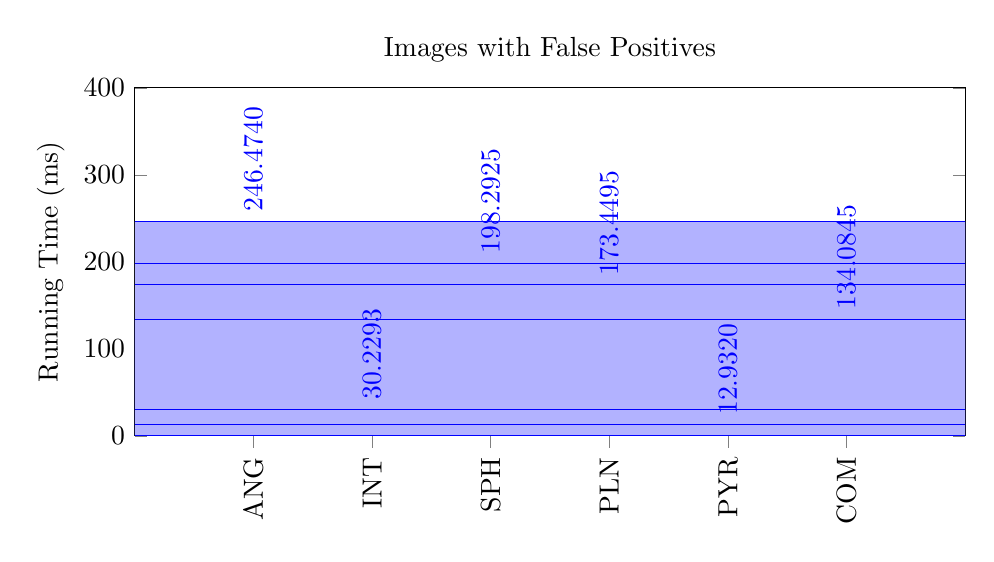
\begin{tikzpicture}
			    \begin{axis}[
			    title={Images with False Positives},
			    ybar,
			    width=\linewidth, height=6cm,
			    ylabel={Running Time (ms)}, ylabel near ticks, ymin=0, ymax=400,
			    ytick={0, 100, 200, 300, 400},
			    xtick={1, 2, 3, 4, 5, 6}, xticklabels={ANG, INT, SPH, PLN, PYR, COM},
			    xmin=0, xmax=7, xtick pos=left,
			    nodes near coords, every node near coord/.append style={rotate=90, anchor=west},
			    bar width=12,
			    every node near coord/.append style={
			    	/pgf/number format/fixed zerofill,
			    	/pgf/number format/precision=4
				},
				xticklabel style = {rotate=90,anchor=east},
			    ]
			    \addplot coordinates { 
			    	(1, 246.474) 
			    	(2, 30.22925)
			    	(3, 198.2925)
			    	(4, 173.4495)
			    	(5, 12.932)
			    	(6, 134.0845) 
			    };
			    \end{axis}
			\end{tikzpicture}
		\end{column}
		\end{columns}
	\end{frame}
	\note{}

	\section{Survey Results}
	\begin{frame}
		\frametitle{What are the results?}
		\smallskip
		\begin{columns}
		\begin{column}{0.3\textwidth}
			\begin{equation*}
				\begin{aligned}
					{}^1 &\{star_1, \ star_2, \ star_3\} \\
					{}^2 &\{star_2, \ star_3, \ star_4\} \\
					{}^3 &\{star_3, \ star_4, \ star_5\} \\
					&\vdots \\
					{}^n &\{star_i, \ star_j, \ star_k\} 
				\end{aligned}
			\end{equation*}
		\end{column}
		\begin{column}{0.3\textwidth}
			\centering{\begin{tikzpicture}[scale=2.5,tdplot_main_coords]
    			\node[color=black, anchor=east, fill=white, xshift=-0.02cm] at (0,0,0) {};
			    \draw[->,color=black,line width=0.02cm] (0,0,0) -- (0.7,0,0) node[anchor=north]{$u_1$};
			    \draw[->,color=black,line width=0.02cm] (0,0,0) -- (0,0.7,0) node[anchor=north]{$u_2$};
			    \draw[->,color=black,line width=0.02cm] (0,0,0) -- (0,0,0.7) node[anchor=east]{$u_3$};
			    
			    \coordinate (O) at (0, 0, 0);
			    \coordinate (I_1) at (0.7, 0.6, 0.3);
			    \coordinate (I_2) at (0.	1, 0.3, 0.7);
			    \coordinate (I_3) at (0.3, 0.7, 0.4);
			
				\draw[color=orange!70, line width=0.02cm](O) -- (I_2);
				\draw[color=orange!70, line width=0.02cm](O) -- (I_3);

			    \filldraw[color=blue] (I_2) circle[radius=0.5pt];					 
			    \filldraw[color=blue] (I_3) circle[radius=0.5pt];
			    
			    \tdplotdefinepoints(0,0,0)(0.3,0.3,0.65)(0.3,0.7,0.4)
			    \tdplotdrawpolytopearc[color=orange!50,line width=0.02cm]{0.6}{yshift=0.2cm,xshift=0.2cm}{\textcolor{black!50}{$\theta$}}
			\end{tikzpicture}}
		\end{column}
		\begin{column}{0.3\textwidth}
			\centering{\begin{tikzpicture}[scale=2.5,tdplot_main_coords]
    			\node[color=black, anchor=east, fill=white, xshift=-0.02cm] at (0,0,0) {$U$};
			    \draw[->,color=black,line width=0.02cm] (0,0,0) -- (0.7,0,0) node[anchor=north]{};
			    \draw[->,color=black,line width=0.02cm] (0,0,0) -- (0,0.7,0) node[anchor=north]{};
			    \draw[->,color=black,line width=0.02cm] (0,0,0) -- (0,0,0.7) node[anchor=east]{};
			    
			    \tdplotsetcoord{P}{\rvec}{\thetavec}{\phivec}
				\tdplotsetrotatedcoords{\phivec}{\thetavec}{0}
				\tdplotsetrotatedcoordsorigin{(P)}
				
			    \draw[tdplot_rotated_coords,->,color=black!70,line width=0.02cm] (0,0,0) -- (.6,0,0) node[anchor=east]{};
			    \draw[tdplot_rotated_coords,->,color=black!70,line width=0.02cm] (0,0,0) -- (0,.7,0) node[anchor=west]{};
			    \draw[tdplot_rotated_coords,->,color=black!70,line width=0.02cm] (0,0,0) -- (0,0,.7) node[anchor=west]{};
			    \node[color=black!70,tdplot_rotated_coords,anchor=east,xshift=0.2cm, yshift=0.6cm, fill=white] at (0,0,0) {$V$};
			    
			    \filldraw[tdplot_rotated_coords, color=blue] (.255,.205,.225) circle[radius=0.3pt]; 
			    \filldraw[tdplot_rotated_coords, color=blue] (.35,.01,.1) circle[radius=0.3pt]; 
			    \filldraw[tdplot_rotated_coords, color=blue] (.01,.35,.155) circle[radius=0.3pt]; 
			    
			    \draw[dashed] (O) -- (P) node[anchor=north east, xshift=0.1cm, yshift=-0.5cm]{$Q$};
			\end{tikzpicture}
			$UQ = V$
			}
		\end{column}
		\end{columns}
		\vspace*{2em}
		
		\begin{columns}
		\begin{column}{0.3\textwidth}
			\parbox{\linewidth}{
				1. Order of image subset selection heavily impacts speed
			}
		\end{column}
		\begin{column}{0.3\textwidth}
			\parbox{\linewidth}{
				2. Angular separation best describes constellations, given noisy image
			}
		\end{column}
		\begin{column}{0.3\textwidth}
			\parbox{\linewidth}{
				3. Rotational based identification is slow
			}
		\end{column}
		\end{columns}
	\end{frame}
	\note{}
	
    \begin{frame}
    	\frametitle{Conclusion \& Questions}
    	\medskip
    	    	
    	\centering{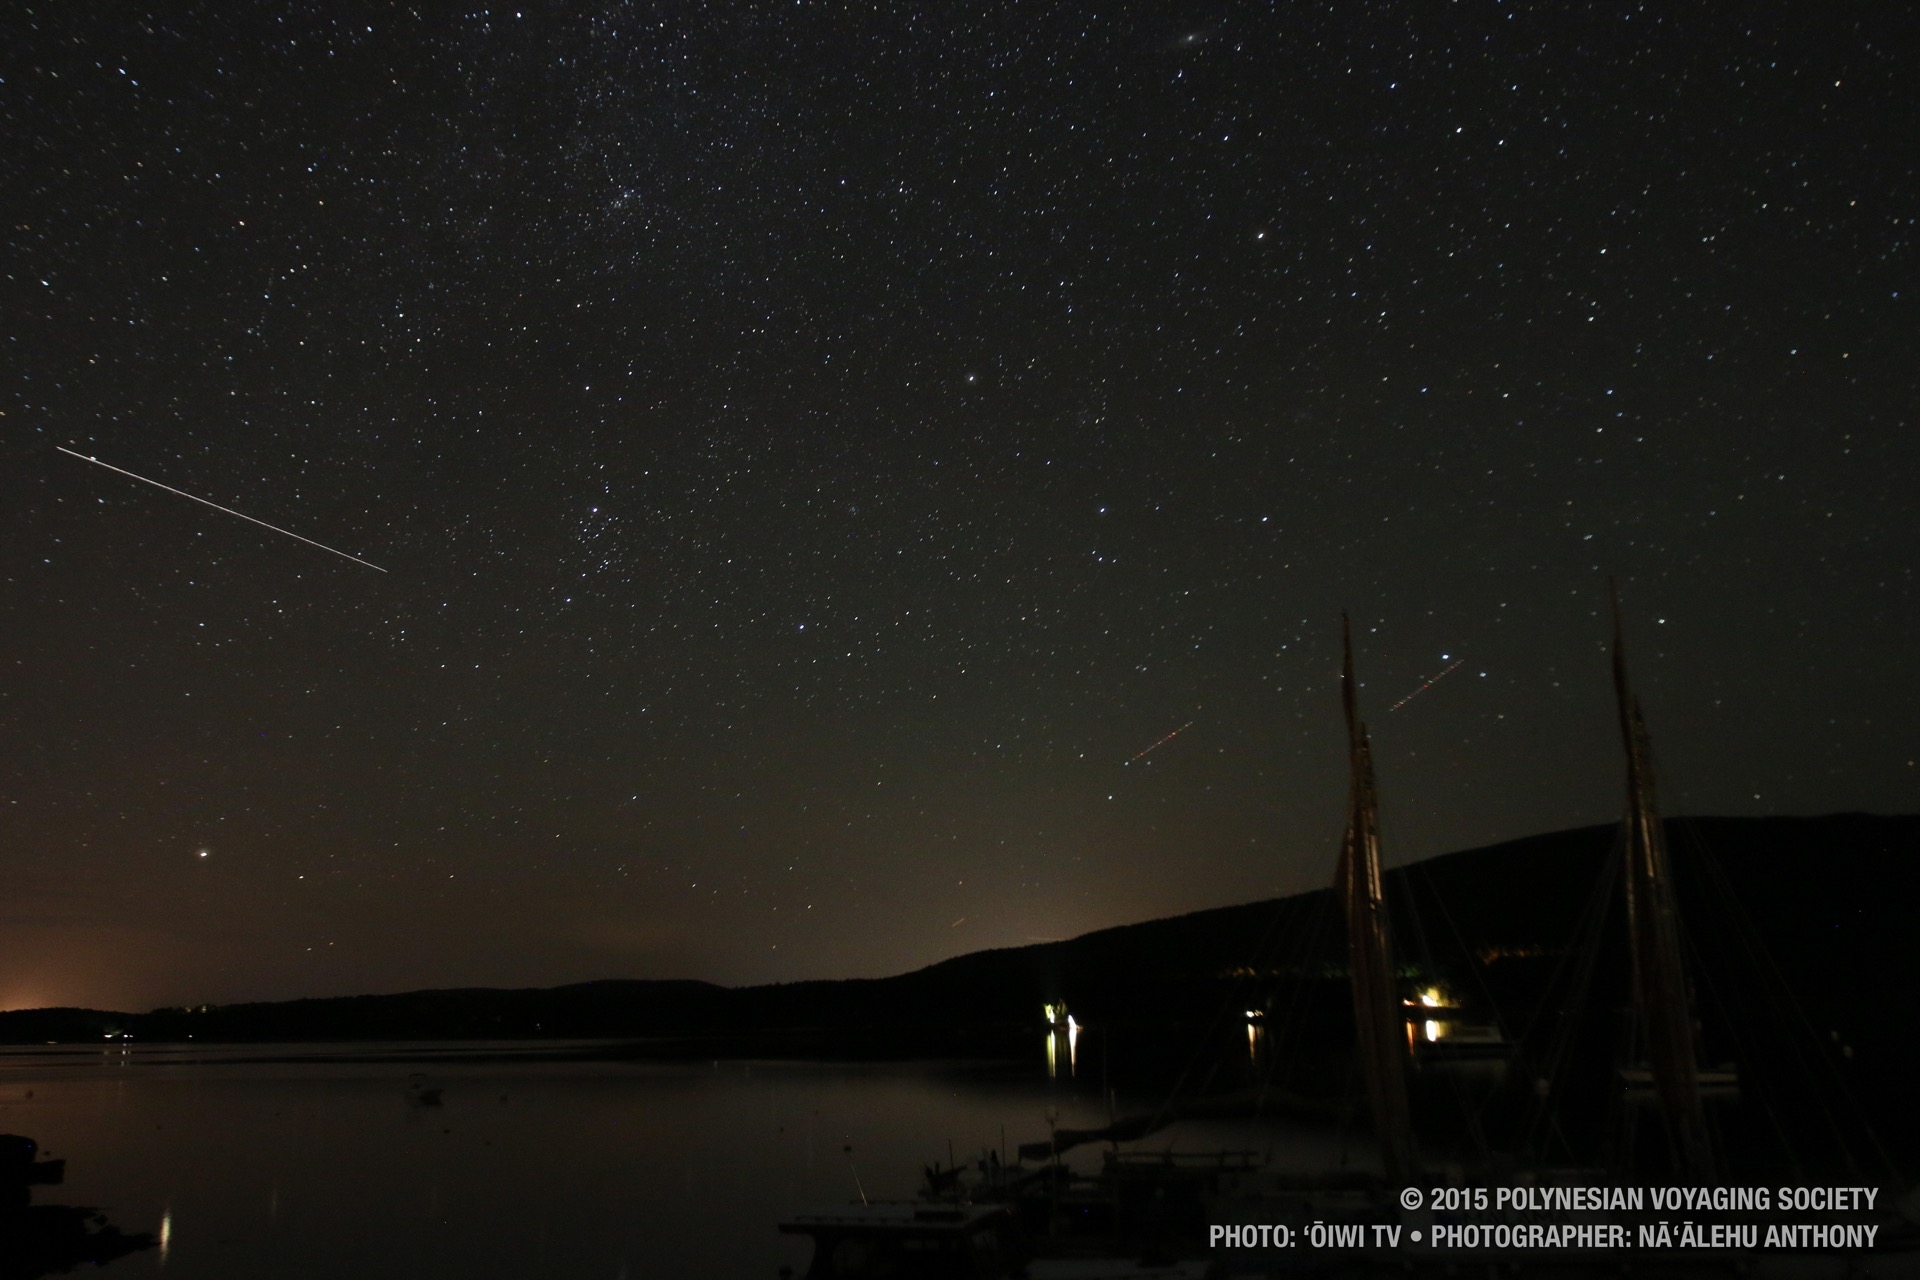
\includegraphics[scale=0.22]{images/hokulea.jpg}}
    \end{frame}
    \note{}

\end{document}
